\chapter{Single Packet Authorization}

Le Single Packet Authorization est le second modèle qui répond à cette problématique. Ce mécanisme repose sur l'envoi, par le client, d'une unique requête au pare-feu.

En suivant ce système, le client va envoyé cette requête contenant un numéro de port. Le pare-feu laissera ensuite passé les paquets émis par le client, à destination du serveur applicatif en utilisant ce port et ce pour une période limitée.

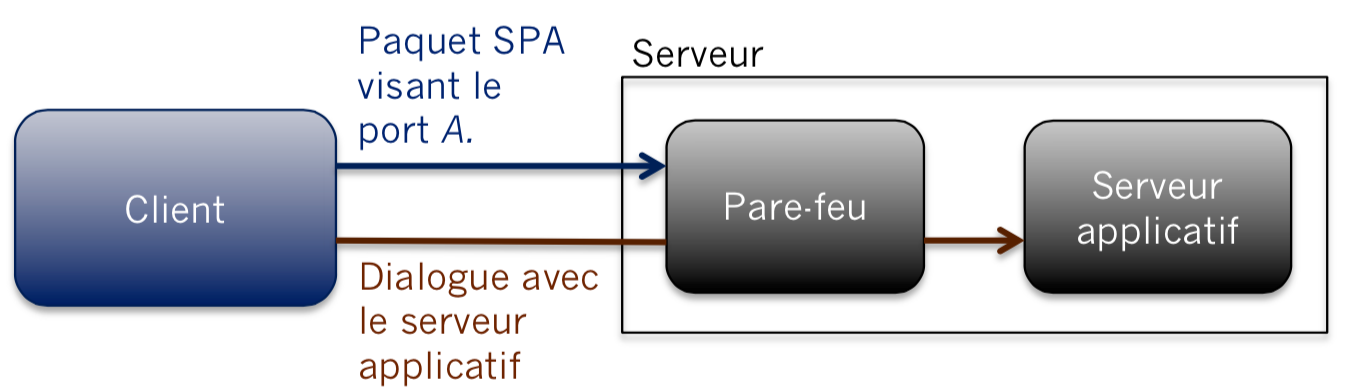
\includegraphics[scale=0.5]{spa_general_1}

Afin que ce mécanisme soit sécurisé, le pare-feu possèdera une clé spécifique à chaque client garantissant ainsi qu'aucune identité ne pourra être usurpée.

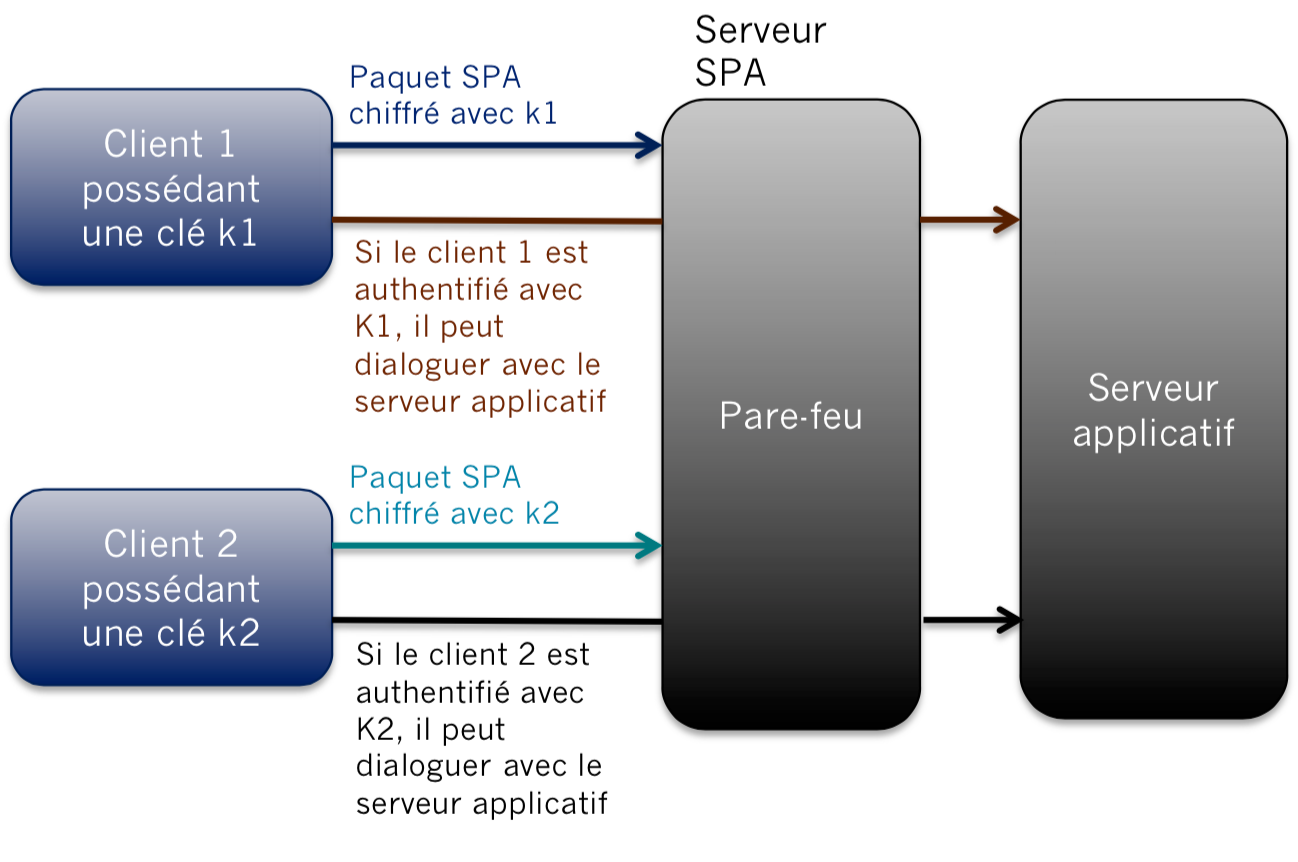
\includegraphics[scale=0.5]{spa_general_2}.

Nous nous proposons d'étudier plus en profondeur cette méthode.
